\documentclass[12pt]{report}
\usepackage[french]{babel}
\usepackage[utf8]{inputenc}
\usepackage{amsmath, amsthm, amssymb, amsfonts}
\usepackage{graphicx}
\usepackage[colorinlistoftodos]{todonotes}
\usepackage{color}
\usepackage{pifont}
\usepackage[Glenn]{fncychap} %Conny, Glenn, Bjarne, Bjornstrup, Rejne, Lenny
\frenchbsetup{StandardLists=true}
%\usepackage[a4paper,pdftex]{geometry}	% Use A4 paper margins
\usepackage[french]{babel}
\usepackage{multicol}
\usepackage[version=3]{mhchem}
\usepackage{hyperref} 
\usepackage[a4paper,pdftex,left=2.5cm,right=2.5cm,top=2.5cm,bottom=2.5cm]{geometry}
\usepackage[section]{placeins} 
\usepackage{float} 
\usepackage{here}
 
 
\definecolor{orange}{cmyk}{0,0.5,1,0}
\definecolor{forestgreen}{rgb}{0.13,0.54,0.13}
\definecolor{carmine}{rgb}{0.59, 0.0, 0.09}
\definecolor{grey}{rgb}{0.5,0.5,0.5}
\definecolor{blue}{rgb}{0.2, 0.2, 0.6}


\begin{document}

\renewcommand{\arraystretch}{1.5}

{\textcolor{carmine}{\chapter{Introduction}}}


{\textcolor{carmine}{\chapter{Analyse de sensibilité}}}

Dans le cadre de la deuxième thématique abordée durant notre projet, à savoir la gestion de la production, il nous a été demandé de faire varier certains paramètres du procédé afin d'analyser leur effet sur : \\
\begin{itemize}
\item La production de $NH_3$, ceci étant notre but premier.
\item Les débits intermédiaires.
\item Le débit de $CO_2$, son caractère polluant étant loin d'être négligeable. Cependant nous avons appris lors de notre visite à Yara\footnote{Dans le cadre du projet, différentes visites ont été proposées. L'une d'elles était la visite du centre de production d'amoniac Yara à Tertre.} qu'il était possible de revendre celui-ci afin de rendre sa production utile. Par exemple dans l'industrie alimentaire. 
\item Le volume d'air à traiter, la séparation de celui-ci étant énergivore et coûteuse.
\end{itemize}

Nous allons faire varier les paramètres suivants dans les plages de valeurs indiquées : \\


\begin{tabular}{|l|c|}
\hline
Rapport $\frac{O_2}{CH_4}$ à l'entrée de l'ATR & 0.2 - 0.8 \\
\hline
Rapport $\frac{H_2O}{CH_4}$ à l'entrée de l'ATR & 0.5 - 4 \\
\hline
Température de sortie de la zone de reforming de l'ATR & 1000 - 1600 [K]\\
\hline
Pression d'opération de l'ATR & 20 - 100 [bar] \\
\hline
\end{tabular}
\bigskip

Pour réaliser notre analyse, nous avons choisi de nous concentrer chaque fois sur une conséquence possible de la variation des paramètres afin de faire clairement ressortir nos possibilités d'action sur ceux-ci.\\
Pour chaque variation, nous avons ressorti les graphes correspondants de notre outil de calcul matlab.\\



\section{Influence sur le débit final de $NH_3$}


\subsection{Variation du ratio molaire $\frac{0_2}{CH_4}$}

Grâce au graphe de la figure 1.1 ci dessous, nous avons pu constater que le débit de $NH_3$ est maximum lorsque le ratio molaire $\frac{O_2}{CH_4}$ est à sa plus petite valeur, c'est à dire $0,2$. Cette valeur implique que la concentration molaire en $CH_4$ soit 5 fois plus élevée que celle en $O_2$.

\begin{figure}[H]
\begin{center}
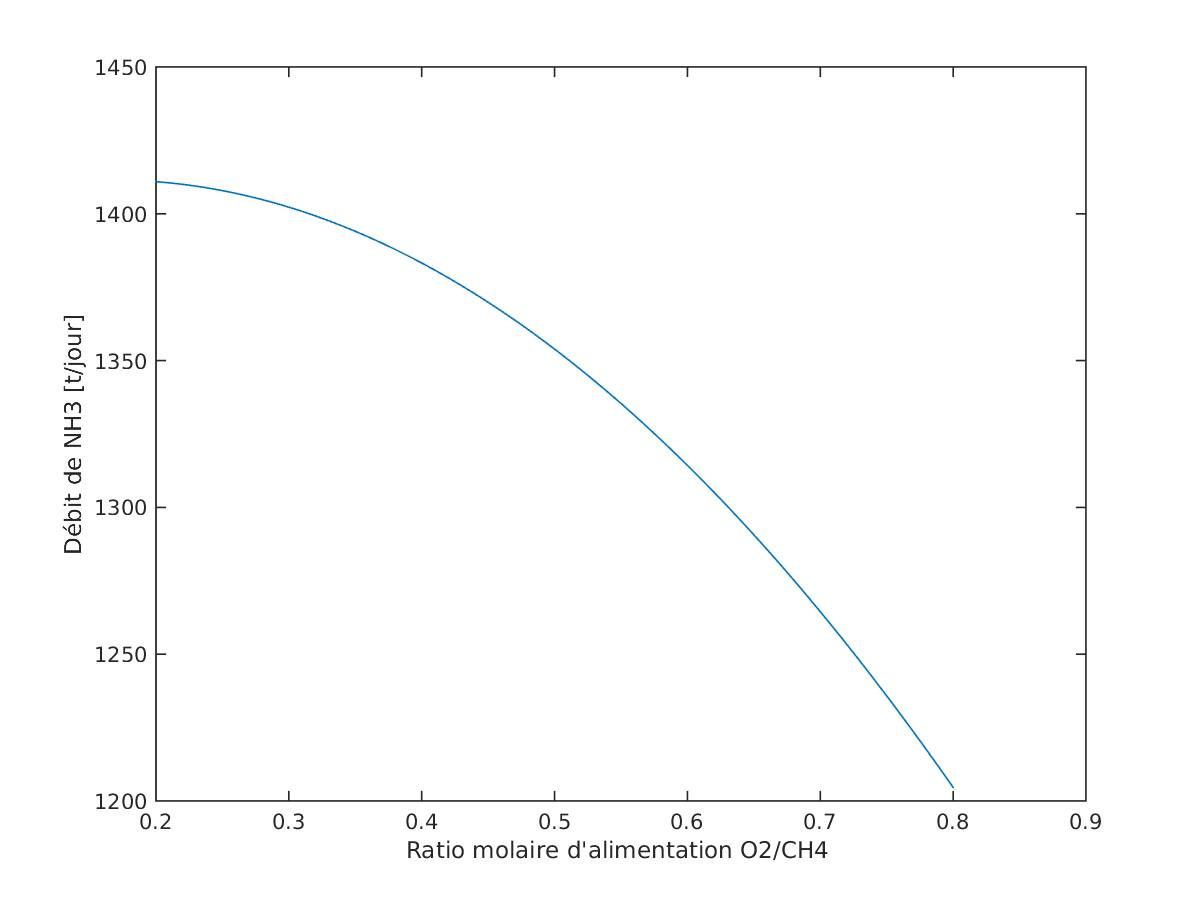
\includegraphics[scale=0.3]{debit_NH3_ratio_O2}
\caption{Evolution du débit de sortie de $NH_3$ en fonction du ratio molaire $\frac{O_2}{CH_4}$}
\end{center}
\end{figure}

Ce phénomène s'explique par le fait que l'$O_2$ n'intervient que dans la toute première réaction dans l'ATR, la combustion, que nous considérons comme complète :

\begin{equation}
 CH_4 + 2O_2 \rightarrow CO_2 + 2H_2O
\end{equation}

 
 Alors que le $CH_4$, quant à lui intervient également dans les deux réactions simultanées :
 
 \begin{equation}
 CH_4 + H_2O \leftrightarrow 3H_2 + CO
 \end{equation}
 \begin{equation}
 CO + 2H_2O \leftrightarrow H_2 + CO_2
 \end{equation}

La réaction (2.1) étant considérée complète, le nombre de moles réagissant est déterminé par le réactif limitant. Dans les plages de valeurs que nous utilisons, ce réactif sera toujours l'$O_2$. Au moins le nombre de moles d'$O_2$ est élevé, au plus il restera du $CH_4$ prêt à réagir avec l'$H_2O$ pour former du $CO_2$ et du $H_2$.\\

Or, le $H_2$ est indispensable à l'étape finale, la synthèse de l'amoniac : 
\begin{equation}
N_2 + 3H_2 \rightarrow 2NH_3
\end{equation}
L'azote, $N_2$, étant obtenu par séparation de l'air et étant 4 fois plus présent dans ce dernier que l'oxygène, est présent en suffisance pour les quantités de $H_2$ prêtes à réagir\footnote{Dans notre outil, selon nos hypothèses}. Dès lors, au plus il y a de $H_2$, au plus nous obtenons du $NH_3$, notre objectif final.\\

Cela explique donc la forme du graphe obtenu.\\

Il est d'ailleurs intéressant de remarquer qu'il est indispensable, pour obtenir du $NH_3$, d'avoir un rapport molaire $\frac{O_2}{NH_3}$ strictement plus petit que 1. Dans le cas contraire, il n'y a pas de $CH_4$ résiduel après la combustion, ce qui empêche la formation de $H_2$ qui est indispensable à la formation de $NH_3$.

\subsection{Variation du ratio molaire $\frac{H_2O}{CH_4}$}

Sur le graphe de la figure 2.2 ci-dessous, il apparaît clairement que le débit de $NH_3$ augmente avec le ratio molaire d'alimentation $\frac{H_2O}{CH_4}$.\\

\begin{figure}[H]
\begin{center}
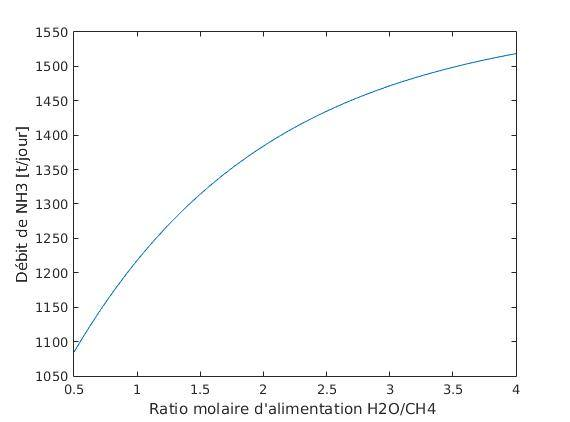
\includegraphics[scale=0.6]{debit_NH3_ratio_H2O}
\caption{Evolution du débit de sortie de $NH_3$ en fonction du ratio molaire $\frac{H_2O}{CH_4}$}
\end{center}
\end{figure}

Cela s'explique principalement par la réaction de formation du $H_2$ qui a lieu dans le WGS : 
\begin{equation}
CO + H_2O \rightarrow H_2 + CO_2
\end{equation}
Etant donné que nous considérons cette réaction comme complète,  c'est le réactif limitant qui détermine le nombre de moles de $H_2$ obtenues et, via l'intervention du $H_2$ dans l'étape finale, la quantité de $NH_3$.\\


\subsection{Variation de la pression dans l'ATR}

\begin{figure}[H]
\begin{center}
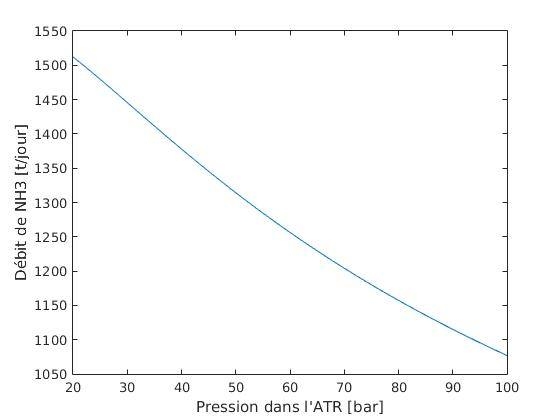
\includegraphics[scale=0.6]{debit_NH3_pression_ATR}
\caption{Evolution du débit de sortie de $NH_3$ en fonction de la pression dans l'ATR}
\end{center}
\end{figure}


\subsection{Variation de la température de la zone de reforming de l'ATR}

\begin{figure}[H]
\begin{center}
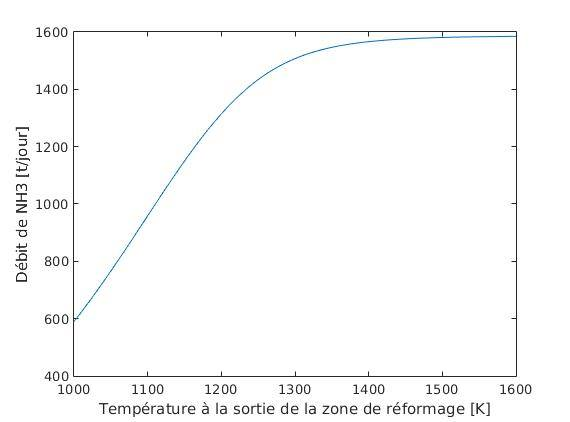
\includegraphics[scale=0.6]{debit_NH3_Temperature}
\caption{Evolution du débit de sortie de $NH_3$ en fonction de la température de la zone de reforming de l'ATR}
\end{center}
\end{figure}



\section{Influence sur le débit de $C0_2$}

\subsection{Variation du ratio molaire $\frac{0_2}{CH_4}$}



\begin{figure}[H]
\begin{center}
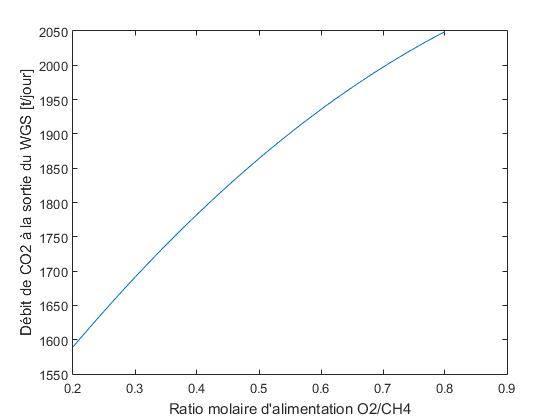
\includegraphics[scale=0.6]{debit_CO2_ratio_O2}
\caption{Evolution du débit de sortie de $CO_2$ en fonction du ratio molaire $\frac{O_2}{CH_4}$}
\end{center}
\end{figure}


\subsection{Variation du ratio molaire $\frac{H_2O}{CH_4}$}


\begin{figure}[H]
\begin{center}
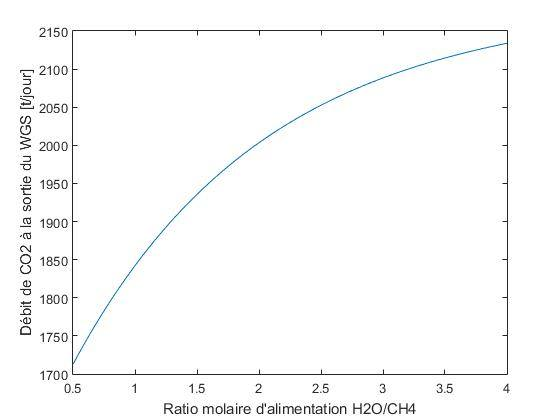
\includegraphics[scale=0.6]{debit_CO2_ratio_H2O}
\caption{Evolution du débit de sortie de $CO_2$ en fonction du ratio molaire $\frac{H_2O}{CH_4}$}
\end{center}
\end{figure}

\subsection{Variation de la pression dans l'ATR}

\begin{figure}[H]
\begin{center}
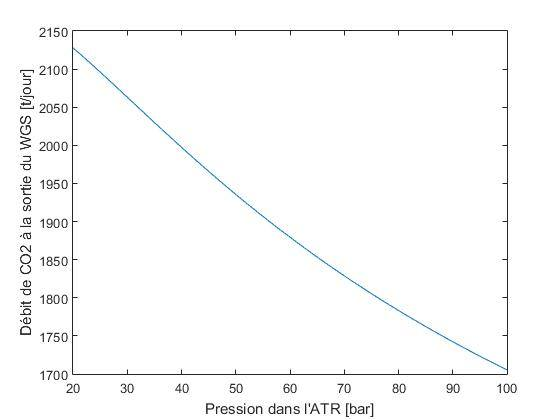
\includegraphics[scale=0.6]{debit_CO2_pression_ATR}
\caption{Evolution du débit de sortie de $CO_2$ en fonction de la pression dans l'ATR}
\end{center}
\end{figure}

\subsection{Variation de la température de la zone de reforming de l'ATR}

\begin{figure}[H]
\begin{center}
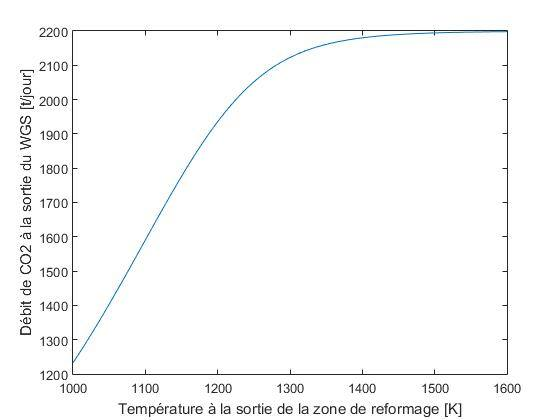
\includegraphics[scale=0.6]{debit_CO2_Temperature}
\caption{Evolution du débit de sortie de $CO_2$ en fonction de la température de sortie de la zone de reforming de l'ATR}
\end{center}
\end{figure}


\end{document}
